% !TEX program = pdflatex
% Continual Learning for Transformer/LLM-Driven Portfolio Optimization Under Non-Stationarity
% Compression-first exposition: one boundary, one spine, minimal proof-of-concept evidence.

\documentclass[11pt]{article}

% -------------------- Layout --------------------
\usepackage[margin=1.0in,top=0.95in,bottom=1.05in]{geometry}
\setlength{\parindent}{0pt}
\setlength{\parskip}{6pt}
\usepackage{microtype}

% -------------------- Math --------------------
\usepackage{amsmath,amssymb,mathtools}

% -------------------- Figures / lists --------------------
\usepackage{graphicx}
\usepackage{caption}
\captionsetup{font=small,labelfont=bf}
\usepackage{xcolor}
\usepackage{enumitem}
\usepackage{placeins}
\setlist[itemize]{leftmargin=*,topsep=2pt,itemsep=1pt,parsep=0pt}

% -------------------- Diagrams --------------------
\usepackage{tikz}
\usetikzlibrary{arrows.meta,positioning,calc}

% -------------------- Links --------------------
\usepackage[hidelinks]{hyperref}

% -------------------- Notation helpers --------------------
\newcommand{\RR}{\mathbb{R}}
\newcommand{\cW}{\mathcal{W}}
\newcommand{\cM}{\mathcal{M}}
\newcommand{\cD}{\mathcal{D}}
\newcommand{\ip}[2]{\langle #1,#2\rangle}
\newcommand{\norm}[1]{\lVert #1\rVert}

% -------------------- Visual system --------------------
\definecolor{Soft}{RGB}{245,247,250}

\tikzset{
  box/.style={draw=black!65,rounded corners,align=center,inner sep=4pt,minimum height=1.8em,fill=white},
  fixed/.style={box,fill=Soft},
  arr/.style={-{Latex[length=2.7mm,width=2.0mm]},line width=0.9pt},
  arrS/.style={-{Latex[length=2.2mm,width=1.7mm]},line width=0.75pt},
  arrCtl/.style={-{Latex[length=2.7mm,width=2.0mm]},line width=0.9pt,dashed},
}

\title{Continual Learning for Transformer/LLM-Driven Portfolio Optimization Under Non-Stationarity\\
\large A constraint-aligned design expressed as one end-to-end spine}
\author{Anonymous (draft for internal planning)}
\date{}

\begin{document}
\maketitle
\vspace{-0.9em}

Online updates are easy to wire up and hard to own. In a portfolio stack, the expensive failures are the quiet ones: a model refresh that looks fine on recent data but changes behavior under stress, pushes the optimizer into corners, or forces you to debug risk after the fact.

We keep this note concrete: a daily-rebalanced, market-neutral, multi-factor US equities long/short portfolio operating through volatility clustering, correlation spikes, and alpha decay. Drift appears as movement in the mapping $(x_t,z_t)\mapsto \mu_t$ from market state $x_t$ and text context $z_t$ to expected \emph{residual} returns.

Throughout---including the toy validation at the end---$\mu_t$ comes from a \textbf{Transformer language model}. Text is tokenized into $z_t$; the Transformer backbone is frozen; and the only parameters we update and ship are a small LoRA adapter.

The interface is intentionally boring. The model may change, but it may only emit an alpha vector $\mu_t$. The decision layer deterministically maps $\mu_t$ to weights $w_t\in\cW_t$, and we only ship an update if it passes a fixed stress suite treated as a regression test. Two invariants hold as $\mu_t$ drifts:
\begin{itemize}
  \item \textbf{Feasibility by construction:} every traded $w_t$ is feasible because it is computed by optimizing over $\cW_t$.
  \item \textbf{Stress non-regression:} an update is rejected if it worsens performance on a fixed stress suite (historical regimes and tail events) treated as a test fixture.
\end{itemize}

\section{Principle: a hard decision boundary}

Trading needs a contract, not a training loop. Each day we take a vector of residual alphas $\mu_t$ and turn it into a portfolio by solving a constrained program. The hard limits live in the optimizer, so they do not depend on the model version.

Each day $t$ after close, we compute target weights $w_t\in\RR^{N_t}$ by solving
\begin{equation}
\label{eq:opt}
\max_{w\in\cW_t}\; \mu_t^\top w\;-\;\tfrac{\gamma}{2}w^\top\Sigma_t w\;-\;c_t^\top|w-w_{t-1}|.
\end{equation}
The important choice is where safety lives: hard limits are encoded in $\cW_t$, not learned.

A minimal production-style feasible set for this spine is
\begin{equation}
\label{eq:Wt}
\cW_t := \Big\{\, w\in\RR^{N_t}:\; \mathbf{1}^\top w=0,\;\norm{w}_1\le L,\;|w_i|\le w_{\max}\;\forall i,\;\norm{w-w_{t-1}}_1\le\tau,\;\norm{B_t^\top w}_\infty\le b_{\text{factor}} \Big\},
\end{equation}
augmented with tail constraints on a fixed scenario library. For stress windows indexed by $j\in\{1,\dots,J\}$ with scenario matrices $R^{(j)}$,
\begin{equation}
\label{eq:es}
\mathrm{ES}_{\alpha}(R^{(j)}w)\ge -L_j\qquad \forall j.
\end{equation}

Problem~\eqref{eq:opt} consumes a learned $\mu_t$ and an auditable risk primitive $\Sigma_t$. In practice, correlations often move faster than alpha, so we treat $\Sigma_t$ as infrastructure and build it from an explicit factor model:
\begin{align}
r_{\tau} &= B_t f_{\tau} + \varepsilon_{\tau},\qquad \tau\in[t-H,t-1],\label{eq:factor_model}\\
\Sigma_t &= B_t\,F_t\,B_t^\top + D_t,\qquad F_t:=\mathrm{Cov}_t(f),\quad D_t:=\mathrm{diag}(\mathrm{Var}_t(\varepsilon_i)).\label{eq:Sigma}
\end{align}

\begin{figure}[t]
\centering
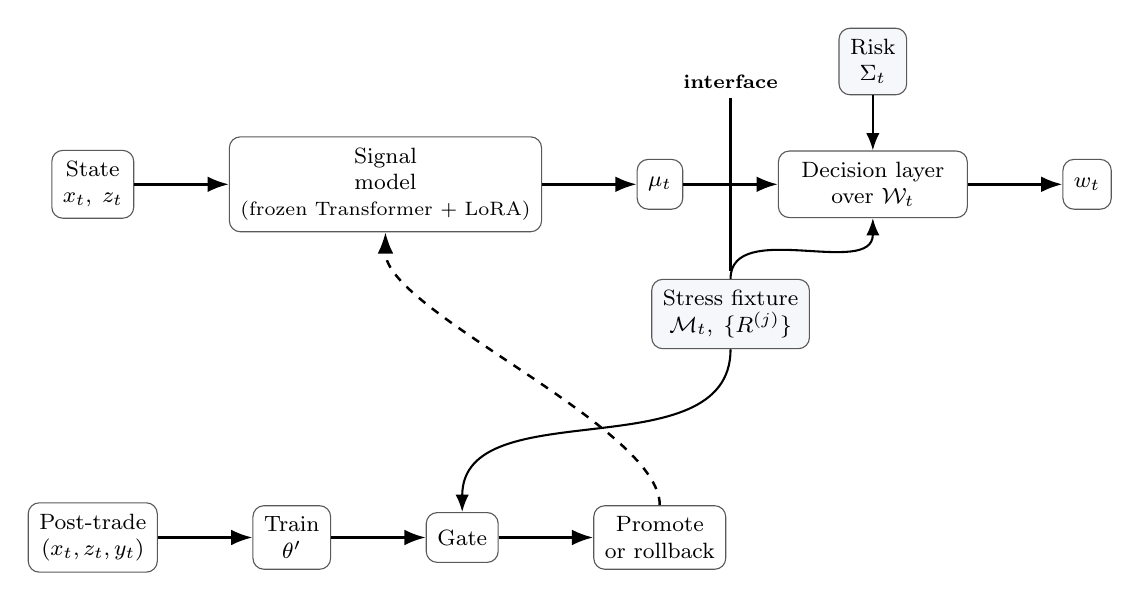
\begin{tikzpicture}[font=\footnotesize, node distance=7mm and 12mm]
  % --- trading plane ---
  \node[box] (state) {State\\$x_t,\;z_t$};
  \node[box, right=of state] (signal) {Signal\\model\\{\scriptsize (frozen Transformer + LoRA)}};
  \node[box, right=of signal] (mu) {$\mu_t$};
  \node[box, right=of mu, minimum width=24mm] (opt) {Decision layer\\over $\cW_t$};
  \node[box, right=of opt] (w) {$w_t$};

  \draw[arr] (state) -- (signal);
  \draw[arr] (signal) -- (mu);
  \draw[arr] (mu) -- (opt);
  \draw[arr] (opt) -- (w);

  % boundary marker: the model outputs $\mu_t$, everything right is deterministic
  \coordinate (bd) at ($(mu.east)!0.5!(opt.west)$);
  \draw[line width=0.95pt] ($(bd)+(0,11mm)$) -- ($(bd)+(0,-11mm)$);
  \node[font=\scriptsize\bfseries, fill=white, inner sep=1pt] at ($(bd)+(0,13mm)$) {interface};

  % fixed primitives
  \node[fixed, above=of opt] (risk) {Risk\\$\Sigma_t$};
  \draw[arrS] (risk) -- (opt);

  \node[fixed, below=12mm of bd] (stress) {Stress fixture\\$\cM_t,\;\{R^{(j)}\}$};
  \draw[arrS] (stress.north) to[out=90,in=-90] (opt.south);

  % --- update plane ---
  \node[box, below=36mm of state] (post) {Post-trade\\$(x_t,z_t,y_t)$};
  \node[box, right=of post] (train) {Train\\$\theta'$};
  \node[box, right=of train] (gate) {Gate};
  \node[box, right=of gate] (swap) {Promote\\or rollback};

  \draw[arr] (post) -- (train);
  \draw[arr] (train) -- (gate);
  \draw[arr] (gate) -- (swap);

  \draw[arrS] (stress.south) to[out=-90,in=90] (gate.north);

  % promotion (reversible swap)
  \draw[arrCtl] (swap.north) .. controls +(up:10mm) and +(down:10mm) .. (signal.south);
\end{tikzpicture}
\caption{\textbf{One interface, two planes.} Trading consumes only $\mu_t$ and enforces feasibility by optimizing over $\cW_t$ with fixed primitives $(\Sigma_t,\{R^{(j)}\})$. Updates are treated like releases: we only promote an adapter if it does not regress on the same audited stress fixture $\cM_t$.}
\label{fig:system}
\end{figure}


If you collapse the boundary, failures stop being legible. Letting the model emit weights turns feasibility into after-the-fact monitoring. Training on raw returns quietly reintroduces factor bets through the back door. Updating large shared parameter blocks without a fixed stress fixture makes rollback expensive and guarantees you will forget rare regimes at exactly the wrong time.

\section{Mechanism: constrained continual updates}

We update only what we can safely roll back: a small LoRA adapter. Two choices keep the update loop aligned with the trading loop: (i) train on residual returns so the model does not relearn factor premia, and (ii) treat the stress suite as a regression test that the update step is not allowed to break.

Residual supervision keeps the learning target stable:
\begin{equation}
\label{eq:resid}
y_t := r_{t+1}-B_t f_{t+1}\in\RR^{N_t}.
\end{equation}
The signal stack predicts expected residual returns $\mu_t=\mu_{\theta}(x_t,z_t)$. The Transformer text backbone is frozen; the only thing we update online is a small LoRA adapter in the head. On the current slice, a simple supervised loss is enough:
\begin{equation}
\label{eq:loss}
\ell_t(\theta)=\sum_{i=1}^{N_t}\big(y_{i,t}-\mu_{i,t}\big)^2.
\end{equation}

Here, ``memory'' is not an abstract task list. It is a fixed test fixture: a curated set of recent points plus stress regimes and edge cases,
\begin{equation}
\label{eq:mem}
\cM_t := \cM_t^{\text{recent}}\;\cup\;\bigcup_{j=1}^J \cM^{\text{stress}(j)}\;\cup\;\cM_t^{\text{edge}}.
\end{equation}
The alignment is structural: the same stress windows define both (a) the replay set we refuse to forget and (b) the scenario library $R^{(j)}$ used in~\eqref{eq:es}.

Each update is allowed to fit the current slice, but it is not allowed to move freely on $\cM_t$. Two stabilizers do the work:
\begin{itemize}
  \item \textbf{Replay distillation (behavior anchor).} Penalize movement away from the deployed model on replay contexts:
  \begin{equation}
  \label{eq:derpp}
  \ell_t(\theta) + \lambda\,\mathbb{E}_{(x,z)\sim\cM_t}\big[\big(\mu_{\theta_t}(x,z)-\mu_{\theta}(x,z)\big)^2\big].
  \end{equation}
  \item \textbf{Gradient projection (hard non-regression).} For stress blocks $\cD^{(j)}\subset\cM_t$ with gradients $g_j=\nabla_\theta \ell_{\cD^{(j)}}(\theta)$, project the current gradient $g_{\text{cur}}$ to satisfy
  \begin{equation}
  \label{eq:gem}
  \min_{v}\;\tfrac12\norm{v-g_{\text{cur}}}^2\quad\text{s.t.}\quad \ip{v}{g_j}\ge -\epsilon_j\;\;\forall j.
  \end{equation}
\end{itemize}
A candidate adapter is promoted only if it passes the fixed gate suite on $\cM_t$; rollback is a single adapter swap.

\section{Evidence: minimal executable validation}

This experiment is intentionally small and opinionated: it is a regression test for the contract above, not a benchmark. The point is to show the failure mode ("tracks drift, forgets stress") and the fix ("adapts without breaking the stress fixture") end to end.

The synthetic market (in \texttt{example\_code/}) simulates $N$ assets with a low-rank factor structure, regime-switching factor covariance, and a regime-dependent alpha mapping, with two forced crisis windows used to define the stress fixture. The testbed is LLM-based: the simulator also emits a token stream whose distribution shifts with regimes; a tiny causal Transformer LM is pretrained once and frozen to produce text embeddings $z_t$.

We compare two update policies with the same frozen Transformer backbone, the same decision layer, and the same initialization: \textbf{naive} (current-slice SGD) vs \textbf{cl} (replay distillation + projected updates + a promotion gate with rollback). We call it a success if stress loss does not regress, IC stays responsive, and the ES budget remains satisfied by construction.

\textit{Reproducibility:} \texttt{python example\_code/run\_validation\_experiment.py} regenerates the embedded figures.

\begin{figure}[t]
\centering
\includegraphics[width=0.49\linewidth]{figures/validation_stress_loss.pdf}\hfill
\includegraphics[width=0.49\linewidth]{figures/validation_ic.pdf}
\caption{\textbf{Core update-loop check.} \textbf{Left:} MSE on a fixed stress fixture (a regression test). Naive online updates eventually forget: stress loss spikes after later drift. Constrained updates stay pinned; $\times$ marks are rejected releases (rollback). \textbf{Right:} 15-day MA of cross-sectional Spearman IC on next-day residuals. The constrained updater stays responsive while protecting the stress fixture.}
\label{fig:val_core}
\end{figure}

\begin{figure}[t]
\centering
\includegraphics[width=0.95\linewidth]{figures/validation_stress_es.pdf}
\caption{\textbf{Feasibility is not a learning problem.} Stress Expected Shortfall on the fixed scenario library (in bp) plotted against the decision-time budget. The trace sits on the budget because the decision layer scales exposure until~\eqref{eq:es} is satisfied; the updater can change $\mu_t$ but it cannot violate $\cW_t$.}
\label{fig:val_es}
\end{figure}

\FloatBarrier

Taken together: Figure~\ref{fig:val_core} shows why the updater must be constrained (stability does not emerge on its own), while Figure~\ref{fig:val_es} shows why feasibility belongs in the optimizer (it stays invariant under model drift).

\end{document}
